\documentclass[conference]{IEEEtran}
\IEEEoverridecommandlockouts
% The preceding line is only needed to identify funding in the first footnote. If that is unneeded, please comment it out.
\usepackage{cite}
\usepackage[portuges,brazil,english]{babel}
\usepackage[utf8]{inputenc}
\usepackage{hyperref}
\usepackage{amsmath,amssymb,amsfonts}
%\usepackage{algorithmic}
\usepackage{graphicx}
\usepackage{textcomp}
\DeclareUnicodeCharacter{00A0}{ }
\def\BibTeX{{\rm B\kern-.05em{\sc i\kern-.025em b}\kern-.08em
    T\kern-.1667em\lower.7ex\hbox{E}\kern-.125emX}}
\begin{document}

\title{Classificador automático de imagens}

\author{\IEEEauthorblockN{André Almeida}
\IEEEauthorblockA{
RA: 164047 \\
\texttt{fda.andre@gmail.com}}
\and
\IEEEauthorblockN{Igor Torrente}
\IEEEauthorblockA{
RA: 169820 \\
\texttt{igortorrente@hotmail.com}}}

\maketitle



\section{Resumo}

Nesse trabalho, estudamos técnicas de aprendizado de máquina e reconhecimento de padrões para obter um modelo eficiente de classificação automática de imagens. Nosso modelo classifica 10 classes de imagens: avião, carro, pássaro, gato, veado, cão, sapo, cavalo, navio e caminhão. As técnicas estudadas variaram de regressão logística até redes neurais artificiais com uma e duas camadas. Durante o estudo coletamos resultados experimentais e chegamos no modelo mais viável dentro das técnicas utilizadas.

\section{Introdução}

\subsection{Classificador automático de imagens}

O problema de classificar imagens vem sendo amplamente estudado pela comunidade acadêmica\cite{b1, b2, b3}. Soluções podem ser aplicadas em diversas áreas do conhecimento, desde biomedicina até segurança pública. Um caso de estudo em destaque é a competição ImageNet\cite{b4}, onde as equipes deveriam, a partir de uma grande banco de dados de imagens classificadas, obter a maior precisão possível com um algoritmo de classificação automática. Em 2012, a competição testemunhou um avanço muito significante: enquanto os campeões de 2010 e 2011 conseguiam, respectivamente, 28\% e 26\% de erro, os pesquisadores conseguiram atingir um erro de 16\% aplicando técnicas de aprendizagem profunda\cite{b5}. A partir de então, todos os ganhadores utilizaram técnicas baseadas nesse mesmo princípio até que em 2015 os ganhadores obteram 3.5\% de erro, ficando abaixo do erro humano.

\subsection{Regressão logística e redes neurais artificiais}

Regressão logística é um modelo empregado em aprendizado de máquina na área de aprendizado supervisionado, comumente  usado para estimar a probabilidade de um exemplo estar em uma classe. Se a chance for maior que 50\%, o modelo diz que esse exemplo faz parte da classe, caso contrário, ele não faz parte. Essa regressão faz uma soma ponderada da entrada e retorna o resultado da função sigmoid dessa soma (um número entre [0,1]).\cite{b6}\\
Rede neural artificial é uma coleção de unidades chamadas neurônios que são interligados entre si com uma ordem (camada), com inspiração biológica no funcionamento do cérebro humano. Cada neurônio de uma camada se liga a todos os neurônios da anterior (se não for a camada de entrada) e da posterior (se não for a camada de saída). Cada neurônio é ativado de acordo com uma função de ativação, os parâmetros dessa função de ativação são as saídas dos neurônios anteriores multiplicados por um peso nas arestas que conectam estes neurônios\cite{b6}.\\ 
Nesse trabalho estamos usando ambas técnicas para fazer experimentos em classificação.
  
\subsection{Base de dados}
A base de dados empregada para treinamento do problema foi a CIFAR-10\cite{b7}, que contêm 60 mil imagens PNG 32x32 coloridas categorizadas nas dez classes que propomos em classificar. Cada imagem então é armazenada em um \textit{numpy array} com 3072 números inteiros, de 0 à 255. Os 3072 representam os 1024 pixels de cada cor RGB. As classes ficam em um vetor de inteiros, onde cada número, de 0 à 9, representa uma classe.

\begin{center}
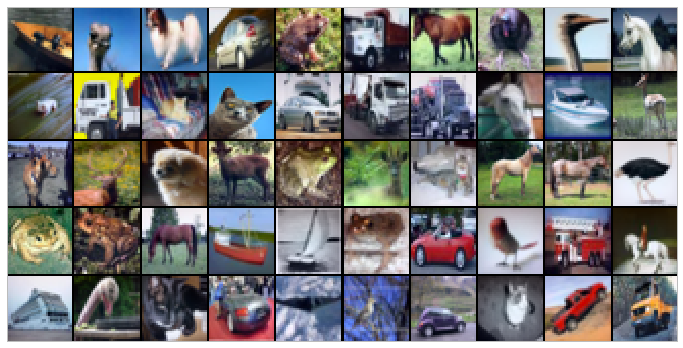
\includegraphics[scale=0.20]{cifar10.png}
\\
\textbf{Figura 1}: \textit{Amostra de imagens do banco}
\end{center}

\subsection{Tecnologias empregadas}
Utilizamos a biblioteca \textit{sklearn}\cite{b8} do \textit{Python} para as chamadas de pre-processamento de dados e treinamento das funções classificadoras. O \textit{Jupyter} foi escolhido como ambiente de desenvolvimento.

\subsection{Infraestrutura computacional}
Os recurso computacionais foram:

\begin{itemize}
\item Computador com um processador Intel Core i7-3537U (2.00GHz × 4) e com 7,7 GiB disponíveis de memória RAM com Arch Linux;

\item Máquina virtual com 4 núcleos virtuais do processor IBM Power8, com 16GB de RAM e  Ubuntu 17.04;

\item Computador com core i5 4440, 8 GB de Ram e Windows 10.

\end{itemize}

\section{Tratamento de dados}

Devido ao tamanho dos dados (um vetor de 3072 inteiros), para obter uma performance melhor, foi aplicada uma redução de dimensionalidade com PCA\cite{b9}. Além disso, como sugerido por\cite{b10}, as bordas da imagem contêm informação menos relevante que o centro, e, além de otimizar as computações, isso também aumentaria a precisão, fazendo o algoritmo focar na parte principal da imagem e com conteúdo relevante.\\
Também foi considerado o uso de LDA, porém nenhum computador conseguiu dispor de memória RAM suficiente na hora do cálculo, tornando inviável essa técnica.\\
Como também será explorado nas seções seguintes, a utilização do PCA gerou resultados melhores e diminui o tempo necessário de processamento. Conforme resultados abaixo, foi adotado aproximadamente 93\% de redução no PCA nos dados das soluções propostas.

\begin{center}

    \begin{tabular}{| l | l | l | l |}
    \hline
    \textbf{\% de PCA} & \textbf{Tempo (s)} & \textbf{Score} \\ \hline
    \textit{Sem PCA} & 1232 & 0.3624 \\ \hline
    85 & 23 & 0.3639 \\ \hline
    93 & 14 & 0.378 \\ \hline
    95 & 18 & 0.3765 \\ \hline
    97 & 41 & 0.3737 \\
    \hline
    \end{tabular}
\newline
    
\textbf{Tabela 1. }\textit{Exemplo de treinos de regressão logística com uso de PCA no mesmo conjunto de dados}

\end{center}

\section{Soluções propostas}
Nessa sessão e nas próximas, score é a métrica de acerto do dado definida na regressão logística\cite{b11, b12} e da  rede neural \cite{b11, b13} como o resultado da função de acurácia\cite{b14}, que é calculada pela razão quantidade de acertos da rede e o número total de amostras testadas, tal como a fórmula abaixo descreve:\\

$acuracia \left (y,y'  \right) = \sum_{i = 1}^{n _{amostra}}{\left \{\begin{matrix}
1 \: ,se \: yi=yi'& \\
0 \: ,se \: yi\neq yi'& 
\end{matrix}\right.}$

\subsection{Regressão logística com um contra todos}
A regressão logística é comumente usado pra classificação binária, seu valor de retorno pode
ser interpretado como uma probabilidade. No caso como temos dez classes usamos a regressão
logística com a estratégia de um versus todos, em que treinamos 10 classificadores binários
que irão dar seu score para cada imagem avaliada, o classificador que dar o maior score 
será o que decidirá a classe da imagem. Para usar a regressão logística nós utilizamos o sklearn.linear\_model.LogisticRegression do sklearn com os parâmetro n\_jobs = -1 e solver="saga" que obtivemos os melhores resultados.

\subsubsection{Sem PCA}
Como descrito acima o melhor resultado foi obtido com o parâmetro solver=\textit{saga} que obtivemos 0.3885 na validação e 0.3938 nos testes.

\subsubsection{Com PCA}
Com PCA de 0.93 que, como visto na tabela 1, gerou o melhor resultado tanto com relação ao tempo computacional quanto ao \textit{score}. Na validação, obtivemos 0.4001 nos testes obtivemos 0.4011 de \textit{score}.


\subsection{Regressão logística multinomial}

A regressão logística multinomial é utilizada para também para classificação multiclasse
mas diferente da regressão logística um versus todos a multinomial suporta múltiplas classes
diretamente usando a função softmax, dada um instancia x ela computa os scores Sk(X) para cada
classe k, então estima a probabilidade de cada classe aplicando a função softmax. Nós utilizamos 
novamente sklearn.linear\_model.LogisticRegression mas com o parâmetro multi\_class='multinomial' do sklearn.

\subsubsection{Sem PCA}
Nós obtivemos um \textit{score} de 0.3893 na validação e 0.3975 nos testes.

\subsubsection{Com PCA}
Nós obtivemos um score de 0.406 na validação e 0.4022 nos testes.

\begin{center}
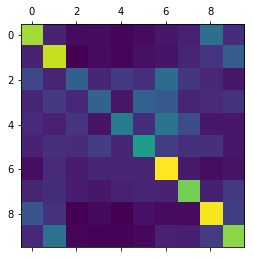
\includegraphics[scale=0.75]{umcontrapca.png}
\\
\textbf{Figura 2}: \textit{Tabela de confusão do modelo multinomial com PCA}
\end{center}

\subsection{Redes neurais artificias com uma camada oculta}

Um modelo relativamente simples de redes neurais conta com apenas uma camada oculta. Nesse modelo, as principais escolhas de hiperparâmetros são: o número de neurônios, a função de custo e a função de ativação. O \textit{momentum} e \textit{learning rate} foram mantidos com o valor padrão do \textit{sklearn}: respectivamente 0.9 e 0.001. Para este treinamento, usamos a função \texttt{sklearn.neural\_network.MLPClassifier}.\\
A função minimizadora de custo lbfgs (algoritmo de Broyden-Fletcher-Goldfarb-Shanno de memoria limitada) é um metodo interativo quase-Newton. A ativação logística (ou sigmoid) é uma função utilizada para introduzir uma "não linearidade" no modelo neural.

\subsubsection{Sem PCA}
Rodamos várias combinações de funções de ativação, funções de custo de números de neurônios. Os resultados dos experimentos podem ser vistos no apêndice. Após uma primeira bateria de testes (Tabela 2) percebemos que a melhor combinação era ativação logística e função de custo \textit{lbfgs}. Rodamos então uma nova bateria de testes, explorando mais essa combinação e chegando no melhor modelo obtido sem PCA foi com a seguinte configuração: 2700 neurônios, função de ativação logística, função de custo \textit{lbfgs}, obtendo um \textit{score} de 0.5109 na validação e \textbf{0.5095} no conjunto de teste.\\

\subsubsection{Com PCA}
Com PCA, os tempos de treino caíram consideravelmente, como esperado. Porém, não conseguimos encontrar um resultado melhor nos testes com validação do que o encontrado nos treinamentos sem PCA, ao contrário do que aconteceu na regressão logística. Após diversos experimentos com um conjunto de validação, chegamos na seguinte configuração: 5000 neurônios, ativação \textit{ReLU} e função de custo \textit{adam}. Os resultados podem ser vistos na tabela 3 no apêndice. O score na validação foi de 0.4399 e nos testes \textbf{0.4814}.

\begin{center}
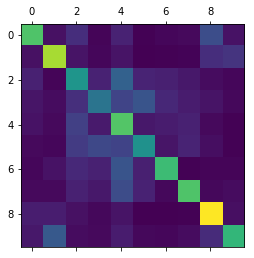
\includegraphics[scale=0.75]{nnsimplespca.png}
\\
\textbf{Figura 3}: \textit{Tabela de confusão do modelo de uma camada com PCA}
\end{center}

A função de ativação ReLU é geralmente a mais recomendada por funcionar bem na prática e tem a vantagem de ser mais rápida computacionalmente.\cite{b6}
\textit{Adam}, um acrônimo de \textit{adaptive moment estimation} é uma função custo que também é recomendada na maioria dos casos e tende a funcionar bem na prática e combina a ideia de duas outras funções de otimização: \textit{Momentum optimization} e \textit{RMSProp}.\cite{b6}

\subsection{Redes neurais artificias com duas camadas ocultas}
Um modelo mais complexo e que permite uma variabilidade maior de parâmetros e resultados é uma rede neural de camada dupla. Com ela, conseguimos modelar melhor cada camada em busca de um modelo mais preciso. Contudo, com isso também aumenta a complexidade computacional e os modelos demoram consideravelmente mais para serem treinados.

\subsubsection{Sem PCA}
Após uma diversidade de testes usando o conjunto de testes sem PCA, notamos um tempo de treinamento muito longo e resultados de scores muito baixos. Os resultados dos testes na validação podem ser vistos no apêndice. O melhor modelo de camada dupla sem PCA teve um score de 0.415 na validação.

\subsubsection{Com PCA}
Com PCA, os treinamentos rodaram de maneira significantemente melhor e puderam ser melhor explorados. O melhor modelo de camada dupla com PCA obteve um score de 0.4736 na validação e tinha 8000 neuronios na primeira camada e 8000 na segunda camada.

\section{Resultados}
  
\subsection{Regressão logística}
Na regressão logística nós obtivemos um aumento significativo do scores e uma diminuição
grande no tempo computacional despendido para o calculo do regressão logística de tanto a normal quanto a multinomial, chegando próximo a 10 vezes em alguns casos. Como visto no item quatro tivemos um aumento do score de 0.3938 para 0.4011 nos testes no caso da regressão logística um contra todos. Mas não houve muita diferença entre os métodos de regressão, obtendo scores muito próximos.

\subsection{Redes neurais artificias}
Apesar do modelo de duas camadas ser mais complexo e admitir mais possibilidades e, apesar do uso de PCA ter se mostrado promissor em regressão logística, o melhor modelo encontrado de redes neurais foi o de uma camada com 2700 neurônios, obtendo um score final de 0.5095. O modelo de duas camadas parecia promissior, porem, conforme os resultados no apêndice, nao encontramos uma combinação que trouxesse resultados relevantes.


\section{Conclusão}
De todos os modelos testados o que obteve o melhor resultado foi a rede neural sem PCA, com 2700 neurônios na camada escondida e com o learning rate de 0.001, que se mostrou superior a alternativa de regressão logística, rede neural com de uma camada com PCA e a rede neural com duas camadas escondidas com PCA. Pela matriz de confusão é possível observar que nosso modelo consegue acertar bem as classes 8 e 2 respectivamente, para um estudo futuro é interessante saber o motivo pelo qual esse modelo acerta mais consistentemente essas classes e não as demais. Com mais mais tempo e poder de processamento acreditamos ser possível melhorar a acurácia do nosso modelo.


\section{Estudos futuros}
Como mostrado em \cite{b15}, para se obter resultados de precisão acima de 75\%, é necessário utilizar outras técnicas que não foram abordadas nesse estudo, como redes convolucionais, aprendizado profundo e redes bayesianas. Um próximo passo do estudo seria analisar essas técnicas e tentar obter resultados melhores do que os obtidos aqui.	


\begin{thebibliography}{00}

\bibitem{b1}Lu, D., \& Weng, Q. (2007). A survey of image classification methods and techniques for improving classification performance. International journal of Remote sensing, 28(5), 823-870.

\bibitem{b2}\texttt{\url{http://rodrigob.github.io/are_we_there_yet/build/classification_datasets_results.html}}

\bibitem{b3}Kang, T. (2015). Using Neural Networks for Image Classification.

\bibitem{b4}\texttt{\url{http://www.image-net.org/challenges/LSVRC/}
}

\bibitem{b5}Krizhevsky, A., Sutskever, I., \& Hinton, G. E. (2012). Imagenet classification with deep convolutional neural networks. In Advances in neural information processing systems (pp. 1097-1105).

\bibitem{b6}  Geron, A. (2017). \textit{Hands-on machine learning with Scikit-Learn and TensorFlow: concepts, tools, and techniques to build intelligent systems.}

\bibitem{b7} \texttt{\url{http://www.cs.toronto.edu/~kriz/cifar.html}}

\bibitem{b8} Scikit-learn: Machine Learning in Python, acessado em 31 de Agosto de 2017, em \texttt{http://scikit-learn.org/stable/index.html}

\bibitem{b9} \texttt{\url{http://scikit-learn.org/stable/modules/decomposition.html\#pca}}

\bibitem{b10} Krizhevsky, A., \& Hinton, G. (2010). Convolutional deep belief networks on cifar-10. Unpublished manuscript, 40.

\bibitem{b11} \texttt{\url{https://github.com/scikit-learn/scikit-learn/blob/ef5cb84a/sklearn/base.py##L322}}

\bibitem{b12} \texttt{\url{http://scikit-learn.org/stable/modules/generated/sklearn.linear_model.LogisticRegression.html}}

\bibitem{b13} \texttt{\url{http://scikit-learn.org/stable/modules/generated/sklearn.neural_network.MLPClassifier.html##sklearn.neural_network.MLPClassifier.score}}

\bibitem{b14} \texttt{\url{http://scikit-learn.org/stable/modules/ model_evaluation.html##accuracy-score}}

\bibitem{b15} \texttt{\url{http://rodrigob.github.io/are_we_there_yet/build/classification_datasets_results.html##43494641522d3130}}

\end{thebibliography}

\section{Apêndices}

\subsection{Resultados dos experimentos com redes neurais artificiais com uma camada}
\subsubsection{Sem PCA}
Usando 80\% do conjunto de treino como treinamento e 20\% como validação. Obtivemos os seguintes \textit{scores} com a função \texttt{MLPClassifier} e seus respectivos parâmetros:

\begin{center}

\begin{tabular}{| l | l | l | l | l |}
\hline
\textbf{Neuronios} & \textbf{Ativação} & \textbf{Func. Custo} & \textbf{Score}  \\ \hline
300       & relu     & adam        & \textbf{0.1003} \\ \hline
300       & logistic & adam        & \textbf{0.1003} \\ \hline
300       & relu     & lbfgs       & \textbf{0.1094} \\ \hline
300       & logistic & lbfgs       & \textbf{0.428}  \\ \hline
1100      & relu     & adam        & \textbf{0.1819} \\ \hline
1100      & logistic & adam        & \textbf{0.1001} \\ \hline
1100      & relu     & lbfgs       & \textbf{0.1163} \\ \hline
1100      & logistic & lbfgs       & \textbf{0.4726} \\ \hline
1900      & relu     & adam        & \textbf{0.1817} \\ \hline
1900      & logistic & adam        & \textbf{0.1447 }\\ \hline
1900      & relu     & lbfgs       & \textbf{0.1554} \\ \hline
\textbf{1900}      & \textbf{logistic} & \textbf{lbfgs}       & \textbf{0.4946 }\\ \hline
\end{tabular} 
\newline
\newline
\textbf{Tabela 2.} \textit{Resultados da seção IV-C-1}
\end{center}

\begin{center}
\begin{tabular}{| l | l | l | l | l |} 
\hline
\textbf{Neurônios}                 & \textbf{Ativação} &\textbf{ Func. Custo} & \textbf{Score}  \\ \hline
100                       & logistic & lbfgs       & \textbf{0.3583} \\ \hline
300                       & logistic & lbfgs       & \textbf{0.4135} \\ \hline
500 					  & logistic & lbfgs       & \textbf{0.4306} \\ \hline
700                       & logistic & lbfgs       & \textbf{0.4602} \\ \hline
900                       & logistic & lbfgs       & \textbf{0.4553} \\ \hline
1100                      & logistic & lbfgs       & \textbf{0.4708} \\ \hline
1300                      & logistic & lbfgs       & \textbf{0.4918} \\ \hline
1500                      & logistic & lbfgs       & \textbf{0.4906} \\ \hline
1700                      & logistic & lbfgs       & \textbf{0.4913} \\ \hline
1900                      & logistic & lbfgs       & \textbf{0.4952} \\ \hline
2100                      & logistic & lbfgs       & \textbf{0.4982} \\ \hline
2300                      & logistic & lbfgs       & \textbf{0.5076} \\ \hline
2500                      & logistic & lbfgs       & \textbf{0.5082} \\ \hline
\textbf{2700}                      & \textbf{logistic} & \textbf{lbfgs}       & \textbf{0.5109} \\ \hline
2900                      & logistic & lbfgs       & \textbf{0.5082} \\ \hline
\end{tabular}
\newline
\newline
\textbf{Tabela 3.} \textit{Resultados da seção IV-C-1}
\end{center}

\subsubsection{Com PCA}
Mesmos testes do item anterior, porém com PCA:

\begin{center}

    \begin{tabular}{| l | l | l | l | l |}
    \hline
    \textbf{Neurônios} & \textbf{Ativação} & \textbf{Func. Custo} & \textbf{Score} & \textbf{Loss} \\ \hline
700                     & relu                   & lbfgs                  & \textbf{0.1827}        &                 \\ \hline
1600                    & relu                   & lbfgs                  & \textbf{0.2204}        &                 \\ \hline
1900                    & relu                   & lbfgs                  & \textbf{0.2393}        &                 \\ \hline
400                     & logistic               & adam                   & \textbf{0.3292}        &                 \\ \hline
100                     & logistic               & adam                   & \textbf{0.3346}        &                 \\ \hline
100                     & relu                   & adam                   & \textbf{0.3348}        &                 \\ \hline
700                     & logistic               & lbfgs                  & \textbf{0.3507}        &                 \\ \hline
400                     & relu                   & lbfgs                  & \textbf{0.3558}        &                 \\ \hline
700                     & logistic               & adam                   & \textbf{0.357}           &                 \\ \hline
1300                    & logistic               & lbfgs                  & \textbf{0.3598}        &                 \\ \hline
400                     & logistic               & lbfgs                  & \textbf{0.3602}        &                 \\ \hline
1000                    & relu                   & lbfgs                  & \textbf{0.3611}        &                 \\ \hline
1000                    & logistic               & lbfgs                  & \textbf{0.3615}        &                 \\ \hline
100                     & logistic               & lbfgs                  & \textbf{0.3675}        &                 \\ \hline
1600                    & logistic               & lbfgs                  & \textbf{0.3687}        &                 \\ \hline
1300                    & relu                   & lbfgs                  & \textbf{0.3713}        &                 \\ \hline
400                     & relu                   & adam                   & \textbf{0.372}           &                 \\ \hline
1000                    & logistic               & adam                   & \textbf{0.3753}        &                 \\ \hline
1900                    & logistic               & lbfgs                  & \textbf{0.3756}        &                 \\ \hline
100                     & relu                   & lbfgs                  & \textbf{0.3825}        &                 \\ \hline
2700                    & logistic               & lbfgs                   & \textbf{0.3863}        &                 \\ \hline
1300                    & logistic               & adam                   & \textbf{0.3872}        &                 \\ \hline
1900                    & logistic               & adam                   & \textbf{0.395}           &                 \\ \hline
1600                    & logistic               & adam                   & \textbf{0.3976}        &                 \\ \hline
700                     & relu                   & adam                   & \textbf{0.3982}        &                 \\ \hline
1000                    & relu                   & adam                   & \textbf{0.4116}        &                 \\ \hline
1300                    & relu                   & adam                   & \textbf{0.4148}        &                 \\ \hline
1600                    & relu                   & adam                   & \textbf{0.4183}        &                 \\ \hline
1900                    & relu                   & adam                   & \textbf{0.4262}        &                 \\ \hline
1700                    & relu                   & adam                   & \textbf{0.3942}        &                 \\ \hline
1800                    & relu                   & adam                   & \textbf{0.3985}        & 1.42108         \\ \hline
2300                    & relu                   & adam                   & \textbf{0.4116}        & 1.58253         \\ \hline
10000                   & relu                   & adam                   & \textbf{0.4118}        & 2.9910          \\ \hline
2200                    & relu                   & adam                   & \textbf{0.4129}        & 1.6623          \\ \hline
5500                    & relu                   & adam                   & \textbf{0.4184}        & 2.26290         \\ \hline
2700                    & relu                   & adam                   & \textbf{0.4182}         & 1.6228         \\ \hline
2000                    & relu                   & adam                   & \textbf{0.42}          & 1.50397         \\ \hline 
4000                    & relu                   & adam                   & \textbf{0.4207}        & 2.7562          \\ \hline
2100                    & relu                   & adam                   & \textbf{0.4234}        & 1.56066         \\ \hline
7500                    & relu                   & adam                   & \textbf{0.4274}        & 2.64004         \\ \hline
6000                    & relu                   & adam                   & \textbf{0.4336}        & 2.2307          \\ \hline
\textbf{5000}           & \textbf{relu}          & \textbf{adam}          & \textbf{0.4399}        & \textbf{1.9009} \\ \hline
    \end{tabular}
\newline
    
\textbf{Tabela 4. }\textit{Resultados da seção IV-C-2}

\end{center}

\subsection{Resultados dos experimentos com redes neurais artificiais com uma camada}

\subsubsection{Sem PCA}
Para simplificar o tamanho da tabela, resultados com \textit{score} abaixo de 0.2 foram omitidos.

\begin{center}
\begin{tabular}{| l | l | l | l | l |}
 \hline
\textbf{Camada 1} & \textbf{Camada 2} & \textbf{Ativação} & \textbf{F. custo} & \textbf{Score}  \\  \hline
100     & 100     & relu     & adam   & 0.2913 \\ \hline
100     & 100     & relu     & lbfgs  & 0.2743 \\ \hline
100     & 100     & logistic & lbfgs  & 0.3253 \\ \hline
100     & 400     & relu     & adam   & 0.262  \\ \hline
100     & 400     & relu     & lbfgs  & 0.2431 \\ \hline
100     & 400     & logistic & lbfgs  & 0.3156 \\ \hline
100     & 700     & logistic & lbfgs  & 0.3186 \\ \hline
100     & 1000    & relu     & lbfgs  & 0.2619 \\  \hline
100     & 1000    & logistic & lbfgs  & 0.3074 \\ \hline
100     & 1300    & relu     & lbfgs  & 0.2714 \\ \hline
100     & 1300    & logistic & lbfgs  & 0.2905 \\ \hline
100     & 1600    & relu     & lbfgs  & 0.2652 \\ \hline
100     & 1600    & logistic & lbfgs  & 0.2893 \\ \hline
100     & 1900    & logistic & lbfgs  & 0.2972 \\ \hline
400     & 100     & relu     & lbfgs  & 0.2643 \\ \hline
400     & 100     & logistic & lbfgs  & 0.3697 \\  \hline
400     & 400     & relu     & lbfgs  & 0.2766 \\ \hline
400     & 400     & logistic & lbfgs  & 0.3868 \\ \hline
400     & 700     & relu     & adam   & 0.2726 \\ \hline
400     & 700     & relu     & lbfgs  & 0.2541 \\ \hline
400     & 700     & logistic & lbfgs  & 0.3744 \\ \hline
400     & 1000    & relu     & lbfgs  & 0.2709 \\ \hline
400     & 1000    & logistic & lbfgs  & 0.3742 \\ \hline
400     & 1300    & relu     & lbfgs  & 0.2849 \\ \hline
400     & 1300    & logistic & lbfgs  & 0.3614 \\ \hline
400     & 1600    & relu     & lbfgs  & 0.3043 \\ \hline
400     & 1600    & logistic & lbfgs  & 0.3615 \\ \hline
400     & 1900    & relu     & lbfgs  & 0.2843 \\ \hline
400     & 1900    & logistic & lbfgs  & 0.367  \\ \hline
700     & 100     & logistic & lbfgs  & 0.3756 \\  \hline
700     & 400     & relu     & adam   & 0.3409 \\  \hline
700     & 400     & logistic & lbfgs  & 0.4129 \\ \hline
700     & 700     & relu     & adam   & 0.3232 \\ \hline
700     & 700     & relu     & lbfgs  & 0.2896 \\ \hline
700     & 700     & logistic & lbfgs  & 0.4057 \\ \hline
700     & 1000    & relu     & adam   & 0.2741 \\ \hline
700     & 1000    & logistic & lbfgs  & 0.4023 \\ \hline
700     & 1300    & logistic & lbfgs  & 0.4062 \\ \hline
700     & 1600    & relu     & lbfgs  & 0.3064 \\ \hline
700     & 1600    & logistic & lbfgs  & 0.3989 \\ \hline
700     & 1900    & relu     & lbfgs  & 0.3077 \\ \hline
700     & 1900    & logistic & lbfgs  & 0.3945 \\ \hline
\textbf{1000}    & \textbf{100}     & \textbf{logistic} & \textbf{lbfgs}  & \textbf{0.415}   \\  \hline
\end{tabular}
\newline
\newline
\textbf{Tabela 5.} \textit{Resultados da seção IV-D-1}
\end{center}

\subsubsection{Com PCA}
Para simplificar o tamanho da tabela, resultados com \textit{score} abaixo de 0.2 foram omitidos.

\begin{center}
\begin{tabular}{| l | l | l | l | l |}
 \hline
\textbf{Camada 1} & \textbf{Camada 2} & \textbf{Ativação} & \textbf{F. custo} & \textbf{Score}  \\  \hline
300  & 600  & relu     & adam  & 0.3681 \\ \hline
300  & 600  & logistic & adam  & 0.3467 \\ \hline
300  & 600  & logistic & lbfgs & 0.3721 \\ \hline
300  & 1400 & relu     & adam  & 0.3796 \\ \hline
300  & 1400 & logistic & adam  & 0.3497 \\ \hline
300  & 1400 & relu     & lbfgs & 0.3551 \\ \hline
300  & 1400 & logistic & lbfgs & 0.3678 \\ \hline
500  & 500  & relu     & adam  & 0.3453  \\ \hline
600  & 1400 & relu     & adam  & 0.3808  \\ \hline
800  & 600  & relu     & adam  & 0.3484 \\ \hline
800  & 600  & logistic & adam  & 0.3554  \\ \hline
800  & 600  & logistic & lbfgs & 0.3436  \\ \hline
800  & 1400 & relu     & adam  & 0.3704  \\ \hline
800  & 1400 & logistic & adam  & 0.349     \\ \hline
800  & 1400 & relu     & lbfgs & 0.3684  \\ \hline
800  & 1400 & logistic & lbfgs & 0.3394  \\ \hline
1400 & 600  & relu     & adam  & 0.3762  \\ \hline
1400 & 600  & logistic & adam  & 0.3777  \\ \hline
1400 & 600  & relu     & lbfgs & 0.3895  \\ \hline
1400 & 600  & logistic & lbfgs & 0.3504  \\ \hline
1400 & 1400 & relu     & adam  & 0.3722  \\ \hline
1400 & 1400 & logistic & adam  & 0.381     \\ \hline
1400 & 1400 & logistic & lbfgs & 0.3529  \\ \hline
1875 & 500  & relu     & adam  & 0.3565  \\ \hline
2000 & 3000 & relu     & adam  & 0.4256  \\ \hline
2000 & 4000 & relu     & adam  & 0.4251  \\ \hline
2000 & 1000 & relu     & adam  & 0.3874  \\ \hline
2000 & 2000 & relu     & adam  & 0.2691 \\ \hline
2000 & 600  & relu     & adam  & 0.3763  \\ \hline
2000 & 600  & logistic & adam  & 0.3867  \\ \hline
2000 & 600  & relu     & lbfgs & 0.3959  \\ \hline
2000 & 600  & logistic & lbfgs & 0.3554  \\ \hline
2000 & 1400 & relu     & adam  & 0.3947  \\ \hline
2000 & 1400 & logistic & adam  & 0.3906  \\ \hline
2000 & 1400 & relu     & lbfgs & 0.3851  \\ \hline
2000 & 1400 & logistic & lbfgs & 0.352     \\ \hline
4000 & 8000 & relu     & adam  & 0.4568  \\ \hline
4000 & 6000 & relu     & adam  & 0.451  \\ \hline
4000 & 3000 & relu     & adam  & 0.4403  \\ \hline
4000 & 4000 & relu     & adam  & 0.4384  \\ \hline
4000 & 1000 & relu     & adam  & 0.408   \\ \hline
6000 & 4000 & relu     & adam  & 0.4615  \\ \hline
6000 & 1000 & relu     & adam  & 0.39    \\ \hline
6000 & 3000 & relu     & adam  & 0.2941  \\ \hline
\textbf{8000} & \textbf{8000} & \textbf{relu}     & \textbf{adam}  & \textbf{0.4736}  \\ \hline
8000 & 6000 & relu     & adam  & 0.4581  \\ \hline
\end{tabular}
\newline
\newline
\textbf{Tabela 6.} \textit{Resultados da seção IV-D-2}

\end{center}
\end{document}
